\documentclass[11pt,usenames,dvipsnames,svgnames,x11names]{beamer}\usepackage[]{graphicx}\usepackage[]{color}
%% maxwidth is the original width if it is less than linewidth
%% otherwise use linewidth (to make sure the graphics do not exceed the margin)
\makeatletter
\def\maxwidth{ %
  \ifdim\Gin@nat@width>\linewidth
    \linewidth
  \else
    \Gin@nat@width
  \fi
}
\makeatother

\definecolor{fgcolor}{rgb}{0.345, 0.345, 0.345}
\newcommand{\hlnum}[1]{\textcolor[rgb]{0.686,0.059,0.569}{#1}}%
\newcommand{\hlstr}[1]{\textcolor[rgb]{0.192,0.494,0.8}{#1}}%
\newcommand{\hlcom}[1]{\textcolor[rgb]{0.678,0.584,0.686}{\textit{#1}}}%
\newcommand{\hlopt}[1]{\textcolor[rgb]{0,0,0}{#1}}%
\newcommand{\hlstd}[1]{\textcolor[rgb]{0.345,0.345,0.345}{#1}}%
\newcommand{\hlkwa}[1]{\textcolor[rgb]{0.161,0.373,0.58}{\textbf{#1}}}%
\newcommand{\hlkwb}[1]{\textcolor[rgb]{0.69,0.353,0.396}{#1}}%
\newcommand{\hlkwc}[1]{\textcolor[rgb]{0.333,0.667,0.333}{#1}}%
\newcommand{\hlkwd}[1]{\textcolor[rgb]{0.737,0.353,0.396}{\textbf{#1}}}%

\usepackage{framed}
\makeatletter
\newenvironment{kframe}{%
 \def\at@end@of@kframe{}%
 \ifinner\ifhmode%
  \def\at@end@of@kframe{\end{minipage}}%
  \begin{minipage}{\columnwidth}%
 \fi\fi%
 \def\FrameCommand##1{\hskip\@totalleftmargin \hskip-\fboxsep
 \colorbox{shadecolor}{##1}\hskip-\fboxsep
     % There is no \\@totalrightmargin, so:
     \hskip-\linewidth \hskip-\@totalleftmargin \hskip\columnwidth}%
 \MakeFramed {\advance\hsize-\width
   \@totalleftmargin\z@ \linewidth\hsize
   \@setminipage}}%
 {\par\unskip\endMakeFramed%
 \at@end@of@kframe}
\makeatother

\definecolor{shadecolor}{rgb}{.97, .97, .97}
\definecolor{messagecolor}{rgb}{0, 0, 0}
\definecolor{warningcolor}{rgb}{1, 0, 1}
\definecolor{errorcolor}{rgb}{1, 0, 0}
\newenvironment{knitrout}{}{} % an empty environment to be redefined in TeX

\usepackage{alltt}

\usepackage{tikz}
\usetheme{Madrid}
\usepackage{amssymb,amsmath,amsthm,amsfonts}
\usepackage{verbatim}
\usecolortheme{whale}
\usepackage[utf8]{inputenc}
\usepackage{polski}
\usepackage{subfigure}
\usepackage{graphicx}

\setbeamertemplate{navigation symbols}{}

\newtheorem{twierdzenie}{Twierdzenie}
\theoremstyle{definition}
\newtheorem{definicja}{Definicja}
\newtheorem{przyklad}{Przykład}
\newtheorem{lemat}{Lemat}
\newtheorem{wniosek}{Wniosek}
\newtheorem{oznaczenia}{Oznaczenia}
\theoremstyle{remark}
\newtheorem{uwaga}{Uwaga}
\IfFileExists{upquote.sty}{\usepackage{upquote}}{}
\begin{document}

%%%%%%%%%%%%%%%%%%%%%%%%%% nowe Marty, Asi i Kasi %%%%%%%%%%%%%%%%%%%%%%%%%%

\begin{frame}
\frametitle{Elastyczność dochodowa -- 4 kategorie dóbr}
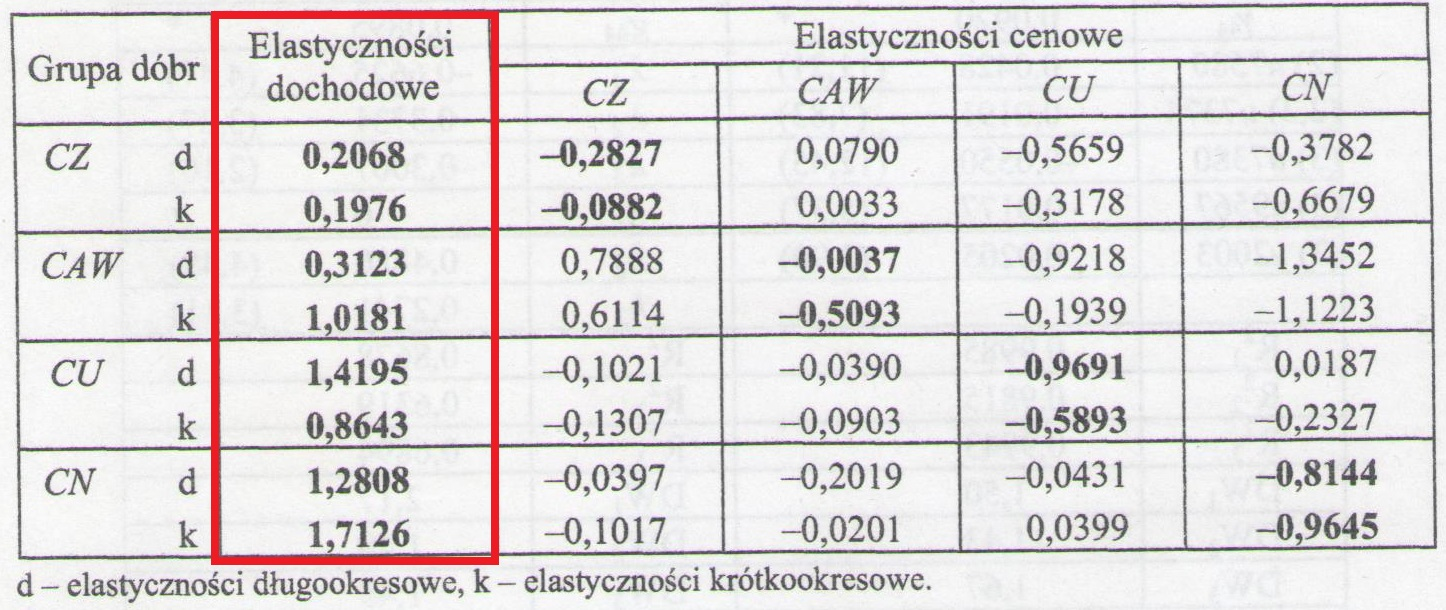
\includegraphics[scale=1]{1.jpg}
\end{frame}

\begin{frame}
\frametitle{Elastyczność cenowa -- 4 kategorie dóbr}
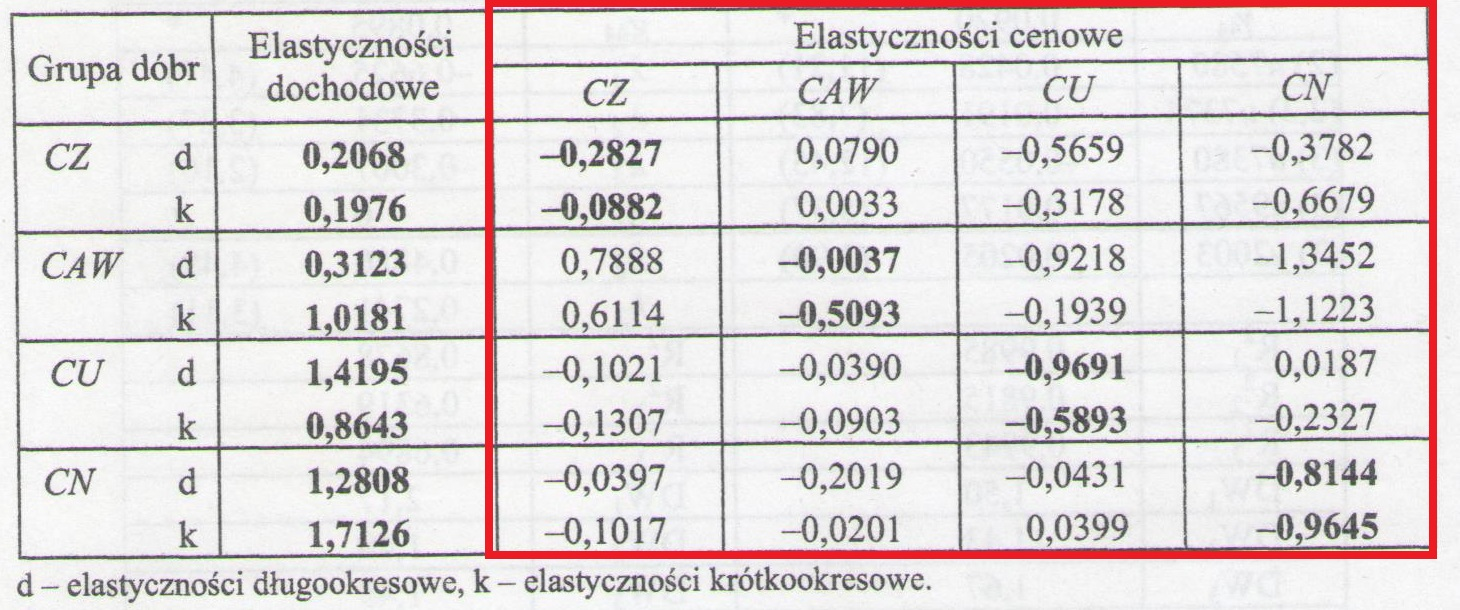
\includegraphics[scale=1]{2.jpg}
\end{frame}

\begin{frame}
\begin{center}
\frametitle{Elastyczność dochodowa -- 12 kategorii dóbr}
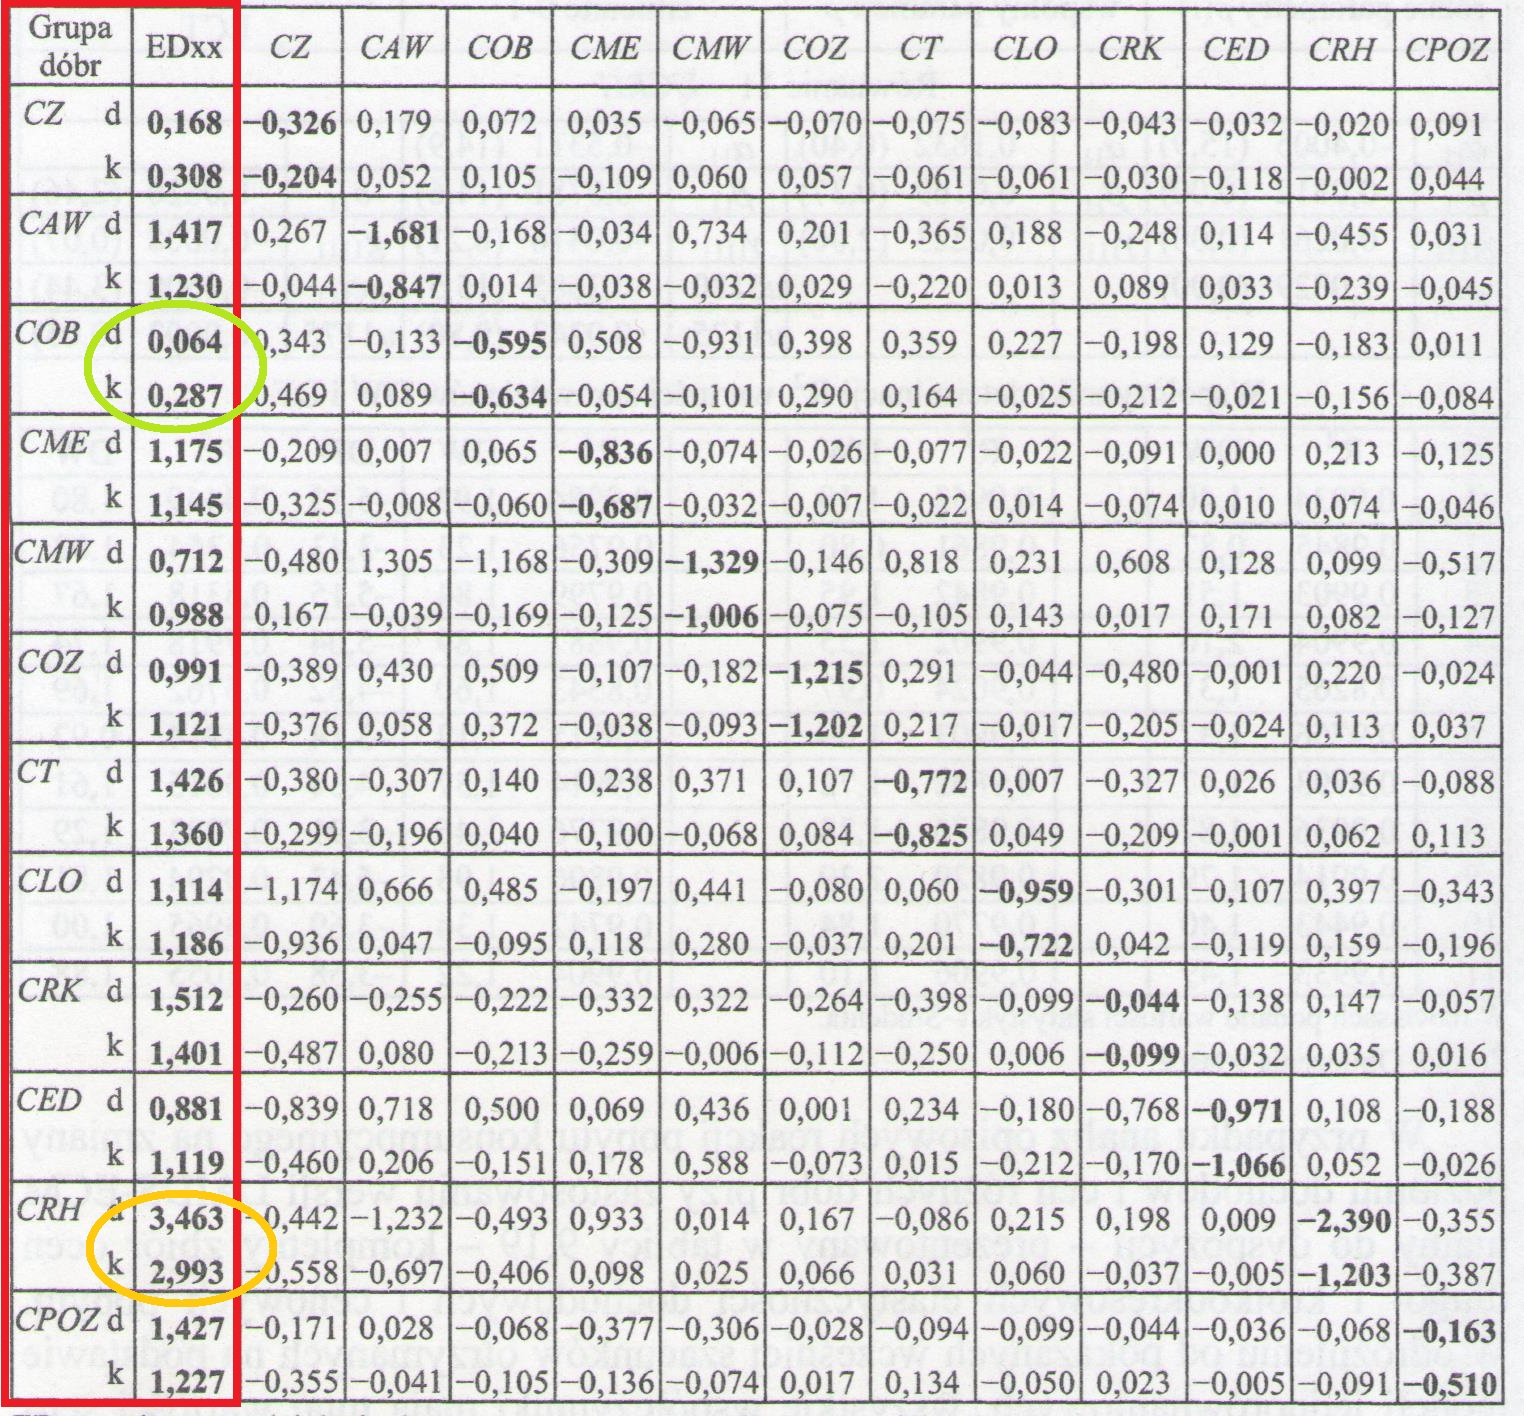
\includegraphics[scale=0.65]{4.jpg}
\end{center}
\end{frame}

\begin{frame}
\begin{center}
\frametitle{Elastyczność cenowa -- 12 kategorii dóbr}
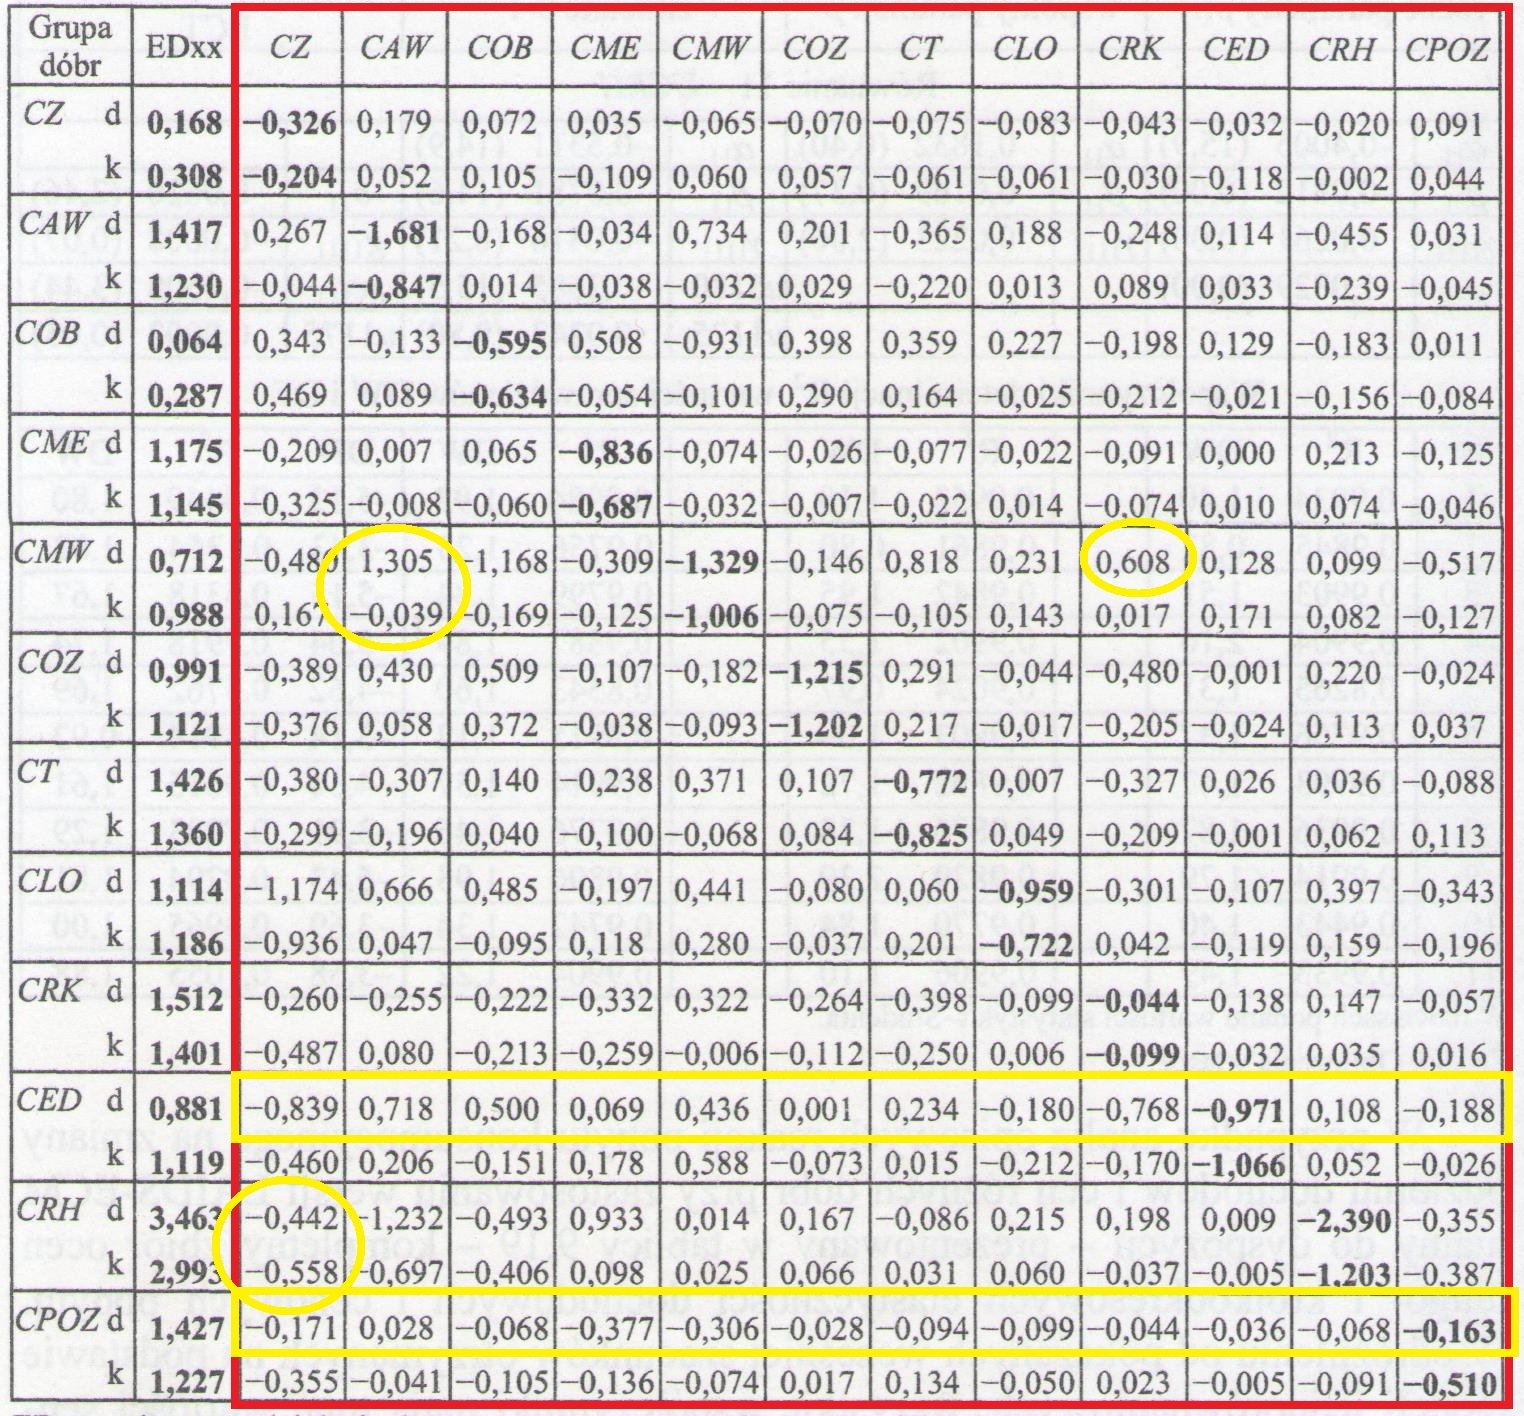
\includegraphics[scale=0.65]{5.jpg}
\end{center}
\end{frame}

\begin{frame}
\begin{center}
\frametitle{Przykład 2}
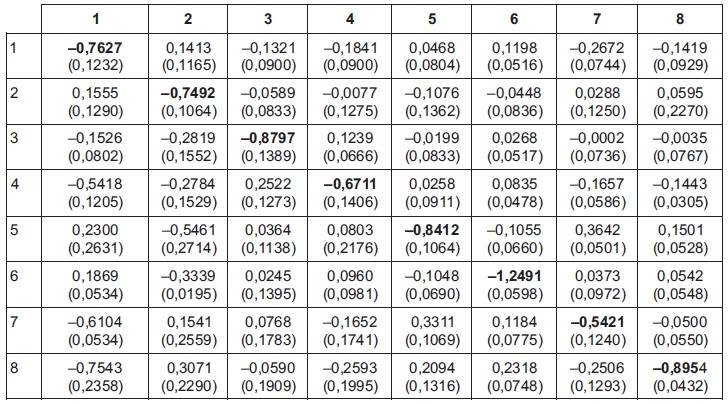
\includegraphics[scale=0.4]{asia.jpg}
\end{center}
\end{frame}

\begin{frame}
\begin{center}
\frametitle{Przykład 3}
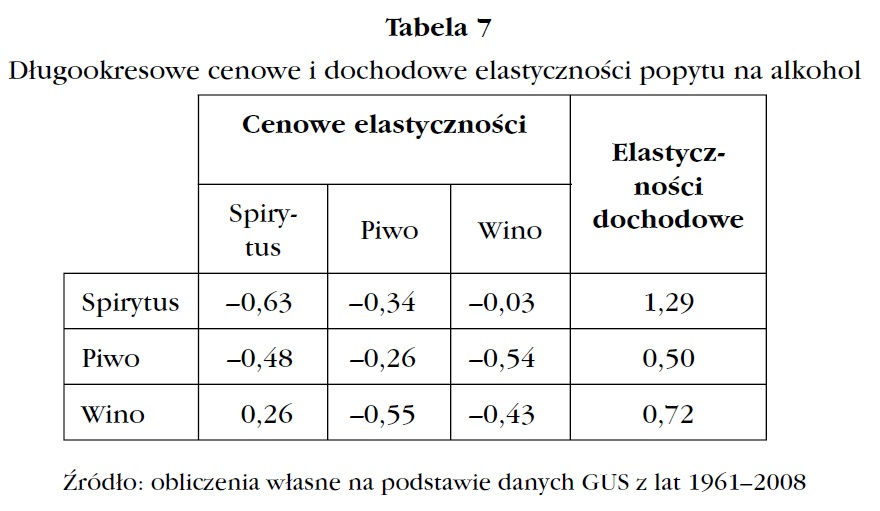
\includegraphics[scale=0.5]{k1.jpg}
\end{center}
\end{frame}

\begin{frame}
\frametitle{Przykład 3}
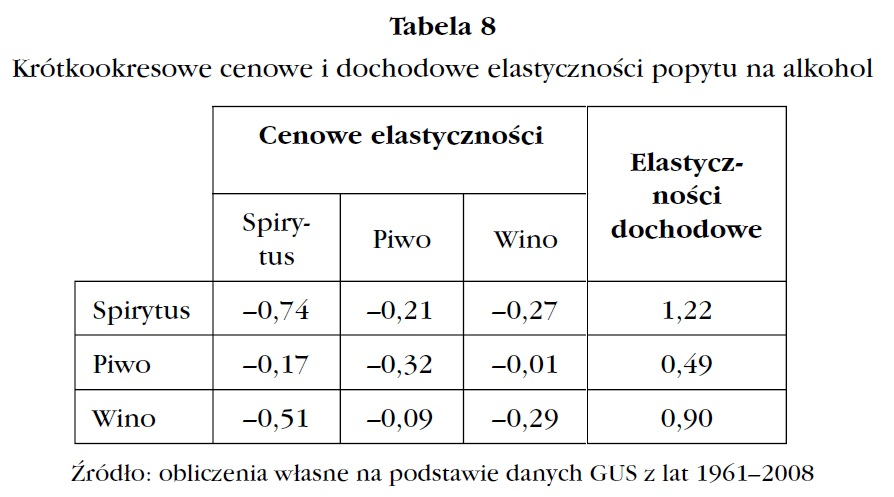
\includegraphics[scale=0.5]{k2.jpg}
\end{frame}

%%%%%%%%%%%%%%%%%%%%%%%%%%%% za to, co jest dalej nie odpowiadam - i tak pewnie wszystko usuniesz :D %%%%%%%%%%%%%%%%%%%%%%%%%%%%%%%%%%%%%%%%%%%%%%



\begin{frame}
\begin{center}
\Huge{MODEL AIDS \\ dla rynku polskiego}

\medskip
\medskip
\medskip

\LARGE{Joanna Czapla \ Katarzyna Grzegrzółka \newline Marta Sommer \ Paulina Sypiańska}
\end{center}
\end{frame}

%%%%%%%%%%%%%%%%%%%%%%%% ASIA %%%%%%%%%%%%%%%%%%%%%%%%%%%%%%%%%%%%%%%%%%%

\begin{frame}
\frametitle{Wyniki estymacji "prawie idealnego" modelu popytu }
Można zauważyć, że w ostatnich 20 latach model "prawie idealny" AIDS stał się bardzo popularnym narzędziem w badaniach popytu. Jego dobre teoretyczne własności, możliwości różnych modyfikacji i zastosowań dla różnych poziomów dezagregacji popytu powodują, iż w wielu pracach i ekspertyzach z zakresu analizy i prognozowania rynku model ten jest z powodzeniem estymowany i stosowany. \newline Ponadto - ze względu na istnienie postaci liniowej LAIDS (linear almost ideal demand system) - możliwe jest tutaj zaprezentowanie metodologii analizy niestacjonarności i modelowania zmiennych skointegrowanych w wielorównaniowych modelach popytu.
 \end{frame}
 
\begin{frame}
\frametitle{Wyniki estymacji "prawie idealnego" modelu popytu }
Przy empirycznej weryfikacji wariantów modelu AIDS analizy i rezultaty estymacji prezentowane będą na dwóch poziomach agregacji, mianowicie dla podziału spożycia całkowitego na cztery kategorie (CZ, CAW, CU, CN) oraz na dwanaście kategorii wydatków (według klasyfikacji COICOP). \newline Podstawową, ogólną nieliniową postać równań modelu "prawie idealnego" NLAIDS można przedstawić następująco: 
$$ w_{it} = (\alpha_{i} - \beta_{i} \alpha_{0}) + \sum\limits_{j} \gamma_{ij} \log p_{jt} + \beta_{i} [ \log m_{t} - \sum\limits_{k} \alpha_{k} \log p_{kt} + $$ 
$$ - \frac{1}{2} \sum\limits_{k}\sum\limits_{j} \gamma_{kj} \log p_{kt} \log p_{jt} ] + \epsilon_{it}, \quad i=1, \ldots , n, $$
\end{frame}
 
\begin{frame}
\frametitle{Wyniki estymacji "prawie idealnego" modelu popytu }

gdzie: \newline $w_{it}$ - udziały wydatków na poszczególne grupy dóbr w wydatkach całkowitych \newline $w_{it} = \frac{p_{it}q_{it}}{m_{t}}$, przy testowanych lub nakładanych na paramatery strukturalne restrykcjach wynikających z trzech warunków teoretycznych: 
\begin{itemize}
\item budżetowego (addytywności) $\sum\limits_{i=1}^{n} \alpha_{i}=1, \qquad \sum\limits_{i=1}^{n} \gamma_{ij} = 0, \qquad \sum\limits_{i=1}^{n} \beta_{i} = 0,$
\item jednorodności stopnia zerowego funkcji popytu $\sum\limits_{j=1}^{n} \gamma_{ij} = 0,$  
\item symetryczności efektów substytucji $\gamma_{ij} = \gamma_{ji}.$
\end{itemize}
\end{frame}

\begin{frame}
\frametitle{Wyniki estymacji "prawie idealnego" modelu popytu }
Mimo iż podejmowane były próby estymacji tego modelu o równaniach nieliniowych  względem parametrów, zdecydowanie większą popularność w zastosowaniach praktycznych ma system o równaniach liniowych LAIDS. Konstrukcja LAIDS wynika z przyjęcia aproksymacji formuły ogólnego indeksu cen z nieznanymi a priori parametrami:
$$ \log P_{t} = \alpha_{0} + \sum\limits_{i} \alpha_{i} \log p_{it} + \frac{1}{2} \sum\limits_{i=1}^{n} \sum\limits_{j=1}^{n} \gamma_{ij} \log p_{it} \log p_{jt}, $$
przez inny indeks cen, którego wartości są z góry ustalone (egzogeniczne). Najczęściej wykorzystuje sie tutaj indeks cen spożycia całkowitego wynikający z makroekonomicznych rachunków konsumpcji (PC=CP/C) lub formułę zastosowaną przez J.R.N. Stone'a (1953):
$$ P_{t}^{*} = exp{\sum\limits_{k=1}{n} w_{kt} \log p_{kt}}. $$
\end{frame}

\begin{frame}
\frametitle{Wyniki estymacji "prawie idealnego" modelu popytu }
Prezentowane dalej rezultaty dla wybranych wariantów i modyfikacji modelu AIDS biorą za punkt wyjścia model LAIDS o następujących równaniach:
$$ w_{it} = \alpha_{0i} + \sum\limits_{j=1}^{n} \gamma_{ij} \log p_{jt} + \beta_{i} \log CL_{t}^{*} + \epsilon_{it}, i=1, \ldots, n, $$
gdzie: $CL_{t}^{*} = \frac{CPL_{t}}{P_{t}^{*}} = \frac{m_{t}}{P_{t}^{*}}$ - wydatek całkowity w cenach stałych (1995 r.) w przeliczeniu na 1 mieszkańca.
\end{frame}


\begin{frame}
\frametitle{Wyniki estymacji "prawie idealnego" modelu popytu }
Oryginalne parametry strukturalne modelu AIDS mają bardzo złożoną interpretację ekonomiczną. Analizując budowę pośredniej funkcji użyteczności stowarzyszonej z tym modelem o następującej postaci:

$$ V(m, \textbf{p}) = \frac{ \log m - (\alpha_{0} +  \sum\limits_{i} \alpha_{i} \log p_{it} + \frac{1}{2} \sum\limits_{i=1}^{n} \sum\limits_{j=1}^{n} \gamma_{ij} \log p_{it} \log p_{jt} )}{ \beta_{0} \prod\limits_{j=1}^{n} p_{j}^{\beta_{j}}} ,$$
jedynie dla parametrów $\alpha_{0}$ i $\beta_{0}$ można znaleźć bezpośrednią interpretację ekonomiczną. Analizując mianowicie okres bazowy, w którym wszystkie zmienne cenowe - indeksy cen - są równe 1, otrzymujemy:
$$ V(m, \textbf{1}) = \frac{\log m - \alpha_{0}}{\beta_{0}}. $$
\end{frame}

\begin{frame}
\frametitle{Wyniki estymacji "prawie idealnego" modelu popytu }
Na skali porządkowej użyteczność równa zeru - $V=0$ - oznacza kontynuację poprzedniego osiągniętego poziomu zadowolenia konsumenta(subsistence). Z kolei $V=1$ otrzymujemy w sytuacji dojścia do maksymalnego zadowolenia (bliss) z zakupu nowego zestawu dóbr przy odpowiednim poziomie dochodu. Wynika z tego, iż $\alpha_{0}$ jest logarytmem dochodu niezbędnego do utrzymania tego samego, osiagniętego już poziomu konsumpcji, a $\beta_{0}$ oznacza różnicę (przyrost logarytmu) dochodów odpowiednio dla tych dwóch sytuacji. Pozostałe parametry strukturalne równań postaci (9.37) i (9.41) nie mają bezpośredniej interpretacji ekonomicznej i dlatego w analizach ekonomicznych stosowane są dla wybranego okresu oszacowania przeciętnych mierników elastyczności dochodowych i cenowych na poszczególne grupy dóbr. 
\end{frame}

\begin{frame}
\frametitle{Wyniki estymacji "prawie idealnego" modelu popytu }
Dla modelu LAIDS wyprowadzone są formuły przybliżone do obliczania wartości mierników elastyczności. Najczęściej stosowane są następujące wzory: \newline 
$ E_{i} = 1 + \frac{\beta_{i}}{w_{it}} $ - elastyczności dochodowe popytu (wydatków) na i-te dobro,
$ e_{ij} = \frac{\gamma_{ij} - \beta_{i}w_{j}}{w_{i}} - \delta_{ij} $ - elastyczności cenowe na i-te dobro, \newline
gdzie: $\delta_{ij} =1$ dla $i=j$, $\delta_{ij} = 0$ dla $i \neq j.$ \newline
Postać estymacyjna równań modelu zawiera zwykle transformacje pozwalające na spełnienie warunku jednorodności stopnia zerowego funkcji popytu $ \sum\limits_{j} \gamma_{ij} = 0.$ Polegają one na zastosowaniu logarytmów cen relatywnych względem ceny kategorii rezydualnej. Ponadto spełnienie warunku budżetowego wymaga pominięcia równania dla tej grupy dóbr. Warunki symetryczności efektów substytucji $\gamma_{ij} = \gamma_{ji}$ są nakładane poprzez odpowiedni zapis estymowanych równań.
\end{frame}


%%%%%%%%%%%%%%%%%%%%%%%%%%%%%% MARTA %%%%%%%%%%%%%%%%%%%%%%%%%%%%%%%%%%%%%%

\begin{frame}
\frametitle{Model SUR dla czterech grup wydatków}

Będziemy zatem analizować następujący model:
$$
w_{it}=\alpha_i+\sum_{j=1}^n\gamma_{ij}\log p_{jt}+\beta_i\log\dfrac{m_t}{p_t}+\varepsilon_{it}
$$
Grupy wydatków:
\begin{enumerate}
\item[] CZ -- żywność i napoje bezalkoholowe
\item[] CAW -- napoje alkoholowe i wyroby tytoniowe
\item[] CN -- nieżywnościowe dobra materialne
\item[] CU -- usługi niematerialne 
\end{enumerate}
\end{frame}

\begin{frame}

\end{frame}

%%%%%%%%%%%%%%%%%%%%%%%%%%%%%%% KASIA %%%%%%%%%%%%%%%%%%%%%%%%%%%%%%%%%%%%%

 \begin{frame}
 \frametitle{Wyniki estymacji "prawie idealnego" modelu popytu }
 Na podstawie prezentowanych rezultatów można zauważyć, iż po zastosowaniu 
kilku zmiennych zero-jedynkowych w równaniu drugim $(u7580, u7374)$ i trzecim $(u7374, u7380, u9567, u2003)$ otrzymano bardzo dobre dopasowanie równań udziałów budżetowych do danych (współczynniki determinacji powyżej 0,98) przy braku autokorelacji składników losowych. Wartości statystyk testu kointegracji DF: $-4.23\ -3.95,\ -4.48$ pozwalają przyjąć, iż zastosowane równania są kointegracyjnymi i reszty poszczególnych równań są zmiennymi stacjonarnymi. 
\end{frame}

\begin{frame}
\frametitle{Wyniki estymacji "prawie idealnego" modelu popytu }
Rezultaty etapu drugiego wydają się również sensowne. Oceny parametrów składników korekty błędem są statystycznie istotnie różne od zera (przy 5-procentowym poziomie istotności) i mają właściwe znaki ($ect_i<0$), choć nie wszystkie oceny efeków krótkookresowych są statystycznie istotnie różne od zera, nawet przy $10$-procentowym poziomie istotności $(b_2, b_3, g_{12})$.\\
Różna od zera ocena współczynnika $a_3$ oznacza, iż w dynamice krótkookresowej popytu na usługi konieczne jest uwzględnienie trendu. Natomiast efekty kształtowania się przyzwyczajeń $h_i$ są istotne w przypadku popytu na napoje alkoholowe i tyton oraz na usługi.\\
O sensowności ekonomicznej rezuttatów estymacji układu ECM świadczą również oceny długo- i krótkookresowych elastyczności dochodowych i cenowych popytu wyznaczone dla okresu $1993-2003$, prezentowane w tablicy $9.15$. 
\end{frame}
 
 % Tablica 9.15
 \begin {frame}
 \frametitle{Wyniki estymacji "prawie idealnego" modelu popytu }
 W przypadku zastosowania reprezentacji typu TECM do modelowania układów wielorównaniowych w warunkach kointegracji procedura estymacji parametrów jest bardziej złożona. Ponadto wymagana jest odpowiednio duża liczba obserwacji ze wzgledu na konieczność uwzględniania rozkładów opóźnień przyrostów wszystkich zmiennych objaśniających w modelu.
 \end{frame}
 
  \begin {frame}
  \frametitle{Wyniki estymacji "prawie idealnego" modelu popytu }
Reprezentację TECM zaproponowaną przez PC.B.Phillipsa w $1991$ r. po raz pierwszy do empirycznej weryfikacji modelu AIDS zastosował C. L.F.Attfeld $(1997)$. \\
Przypomnijmy, iż po pozytywniej weryfikacji hipotez, że wszystkie zmienne w modelu są zintegrowane stopnia pierwszego $I(1)$, "trójkątny" model korekty błędem TECM mozna zapisać w postaci dwóch bloków równań:
\end{frame}

\begin{frame}
\frametitle{Wyniki estymacji "prawie idealnego" modelu popytu }
\begin{enumerate}
\item zasadniczego układu równań równowagi długookresowej dla zmiennych endogenicznych:
$$ y=Bx+\epsilon $$
gdzie

\begin{itemize}
\item y - wektor zmiennych objaśnianych,
\item B - macierz parametrów $(n\times k)$ dla $n$ równań i $k$ zmiennych objaśniających,
\item t - składniki losowe reprezentujące krótkookresowe odchylenia od stanu równowagi.
\end{itemize}

\item układu dodatkowego dla zmiennych egzogenicznych:
$$ \Delta x=A_1 \Delta x_{t-1} + A_2 \Delta x_{t-2}+...+A_k \Delta x_{t-k} + \xi$$
gdzie
\begin{itemize}
\item $A_i$ - macierze parametrów przy kolejnych opóźnionych przyrostach zmiennych objaśnających.
\end{itemize}
\end{enumerate}
 \end{frame}
 
 \begin{frame}
 \frametitle{Wyniki estymacji "prawie idealnego" modelu popytu }
Przy założeniach rozkładu normalnego składników losowych $\epsilon$ i $\xi$  parametry strukturalne (B) modelu można oszacować albo przy zastosowaniu metody największej wiarygodności, albo modyfikując równania układu zasadniczego poprzez uwzglądnienie rozkładu opóźnień zmiennych 
objaśniających:
$$ y=Bx+\sum_{i=0}^{k}A_i \Delta x_{t-i}+ u_i $$
i zastosowanie wieowymiarowej metody najmniejszych kwadratów.\\
Składowe rozkładu opóźnień przyrostów zmiennych objaśniających traktowane są jako czynniki zakłócające, które można interpretować podobnie, jak składniki losowe modelu.
\end{frame}
 
\begin{frame}

\frametitle{Wyniki estymacji "prawie idealnego" modelu popytu }

Podstawowym problemem zastosowania modelu TECM jest ustalenie rzędu długości opóźnień dla układu $(9.47)$. Ponieważ układ ten można traktować oddzielnie jako klasyczny model VAR dla pierwszych różnic zmiennych, istnieje możliwość zastosowania testu długości opóźnień opierającego się na statystyce współczynnika (ilorazu) wiarygodności LRS.\\
Badanie rozpoczyna się od przyjęcia takiej samej długości opóźnienia, które jest albo najbardziej prawdopodobne, albo najdłuższe z możliwych ze względu na wielkość próby. Weryfikowana jest hipoteza: \\
$H_0:$  długość opóźnień zmiennych wynosi $k-r$   \\
przy hipotezie alternatywnej:\\
$H_1:$  długość opóźnień zmiennych wynosi $k$  \\
gdzie:
\begin{itemize}
\item k-maksymalna długość opóźnienia, od której rozpoczyna się badanie,
\item r-liczba opóźnień, o które chcemy zredukować model.
\end{itemize}
\end{frame}

\begin{frame}
\frametitle{Wyniki estymacji "prawie idealnego" modelu popytu }
Statystyka współczynnika wiarygodności z poprawką Simsa testująca hipotezę, czy długość opóźnienia rzędu $k-r$ jest odpowiednia dla wszystkich równań jednocześnie, ma postać:
$$ LRS=(T-c) (\ln | \sum_{k-r} | - \ln \sum_{k})  $$
gdzie:
\begin{itemize}
\item T-liczba dostępnych obserwacji,
\item c-liczba parametrów estymowanych w każdym z równań nieograniczonego (z maksymalną liczbą opóźnień) modelu VAR,
\item $\ln | \sum_{k} | $ -logarytm naturalny z wyznacznika macierzy 
$ \sum_{k}$ (wariancji-kowariancji reszt dla układu z liczbą opóźnień równą $k$ ),
\item $\ln | \sum_{k-r} | $ -logarytm naturalny z wyznacznika macierzy 
$ \sum_{k-r}$ (wariancji-kowariancji reszt dla układu z liczbą opóźnień równą $k-r$ ).

\end{itemize}
\end{frame}

\begin{frame}
\frametitle{Wyniki estymacji "prawie idealnego" modelu popytu }
Statystyka LRS ma asymptotyczny rozkład $ \chi ^2 $ z liczbą stopni swobody $ \nu=(k-r) \times n^2 $ równą liczbie ograniczeń nałożonych w całym systemie. Jeśli obliczona wartość statystyki jest mniejsza od wartości krytycznej, to nie można odrzucić hipotezy zerowej. Wartości większe od wartości krytycznych powodują odrzucenie hipotezy zerowej na korzyść alternatywnej.
\end{frame}

\begin{frame}
\frametitle{Wyniki estymacji "prawie idealnego" modelu popytu }
W przypadku prezentowanych badń dla Polski, ze względu na ograniczoną do $31$ liczbę obserwacji, testowano maksymalną długość opóźnienia $k=4$.
\\
Postawiono zatem zespół hipotez: \\
 $H_0:$ długość opóźnień zmiennych wynosi $3$,    \\
 $H_1:$ długość opóźnień zmiennych wynosi $4$.   
\end{frame}

\begin{frame}
\frametitle{Wyniki estymacji "prawie idealnego" modelu popytu }
W celu przetestowania hipotez oszacowano parametry dwóch modeli w obrębie tej samej próby:
$$\Delta x_t=A_1 \Delta x_{t-1} + A_2 \Delta x_{t-2}+A_3 \Delta x_{t-3} +\xi_{(3)},$$
$$\Delta x_t=A_1 \Delta x_{t-1} + A_2 \Delta x_{t-2}+A_3 \Delta x_{t-3}+A_4 \Delta x_{t-4} +\xi_{(4)},$$
gdzie: $\Delta x=[dln(CL^*) \ dln(PCZN) \ dln(PCAWN) \ dln(PCUN)]$, a następnie obliczono wartość statystyki współczynnika wiarygodności:
$$LRS=(T-c)(\ln|\Sigma_3|-\ln|\Sigma_4|)=(31-16)(1,006)=15,095.$$
Ponieważ obliczona wartość jest mniejsza od wartości krytycznych rozkładu $\chi^2$ dla 31 obserwacji 
($\chi^2_{\alpha=0,1} \approx 43,8; \ \chi^2_{\alpha=0,05} \approx 50,9 $) nie mamy podstaw do odrzucenia hipotezy zerowej.
\end{frame}
 
\begin{frame}

\frametitle{Wyniki estymacji "prawie idealnego" modelu popytu}

Ze względu na bardzo wysokie wartości współczynników determinacji i brak autokorelacji składników losowych, rezultaty estymacji modelu LAIDS-TECM-3 pokazane w tablicy 9.16 należy uznać za zadowalające. Duża część parametrów stojących przy opóźnionych zmiennych objaśniających ($c_{ij},d_{ij},f_{ij},h_{ij}$) nie rózni się istotnie od zera przy 5-procentowym poziomie istotności. Są to jednak tylko oceny składników zakłócających, więc można przyjąć, iż nie powoduje to zmniejszenia wartości analitycznej i predyktywnej tej wersji modelu "prawie idealnego".  \\

Oceny współczynników elastyczności dochodowych oraz prostych i mieszanych elastyczności cenowych z modelu "trójkątnego" zestawione w tablicy 9.17 mają wartości zbliżone do analogicznych ocen obliczonych dla modelu statycznego, czyli dla relacji długookresowych.
%tabela 9.16
\end{frame}
 %tabela 9.17
 
\begin{frame}
\frametitle{Wyniki estymacji "prawie idealnego" modelu popytu }
Ze względu na dużą liczbę parametrów, które należy oszacować łącznie, zastosowanie modelu TECM jest jednak ograniczone dla dość wysokiego poziomu agregacji dóbr. Dlatego też, w przypadku podziału ogólnego spożycia na dwanaście kategorii, czyli przy empirycznej weryfikacji modelu składającego się z jedenastu niezależnych równań, w tablicy 9.18  prezentowane są rezultaty estymacji tylko modeli typu LAIDS-11 oraz LAIDS-ECM-11.
\end{frame}

\begin{frame}
\frametitle{Wyniki estymacji "prawie idealnego" modelu popytu }
W tablicy 9.18 w celu umożliwienia dokonania własnych, szczegółowych porównań zamieszczono wszystkie rezultaty przeprowadzonych eksperymentów estymacyjnych na tym modelu. Można więc porównywać oceny odpowiednich parametrów uzyskane zarówno dla postaci oryginalnej bez korekt (UWMNK), jak i przy zastosowaniu estymacji UWMNK z uwzględnieniem:
\begin{itemize}
\item różnych współczynników autokorelacji reszt w równaniach modelu (LAIDS-A-11)
\item tego samego współczynnika autokorelacji reszt dla wszystkich równań (LAIDS-R-11)
\item zmiennych zerp-jedynkowych do kontroli zmian wyrazu wolnego i obserwacji nietypowych w niektórych równaniach (LAIDS-Z-11)
\item opóźnionych o jeden okres wektorów reszt do uzyskania ocen efektów krótkookresowych (procedura Engla-Grangera, LAIDS-ECM-11)
\end{itemize}

\end{frame}

\begin{frame}
\frametitle{Wyniki estymacji "prawie idealnego" modelu popytu }
Ze względu na różnorodne możliwości dalszych badań modelu "prawie idealnego" w zastosowaniach do analiz i prognoz popytu na rynkach lokalnych, krajowych i międzynarodowych przy różnych poziomach dezagregacji oraz w dużym zakresie również ze względu na pewną unikatowość badań przeprowadzonych w niniejszej pracy, pozostawiamy wiele problemów otwartych-wymagających dalszych poszukiwań naukowych.\\
W zakończeniu prezentacji rezultatów obliczeń należy jednak ponowanie zwrócić uwagę na praktyczne możliwości zastosowań modelu AIDS.
\end{frame}

\begin{frame}%strona ostatnia (287)
\frametitle{Wyniki estymacji "prawie idealnego" modelu popytu }
W przypadku analiz opisowych reakcji popytu konsumpcyjnego na zmiany poziomu dochodoów i cen różnych dóbr przy zastosowaniu wersji LAIDS-ECM mamy do dyspozycji - prezentowany w tablicy 9.19 - kompletny zbiór ocen długo- i krótkookresowych elastyczności dochodowych i cenowych popytu. W odróżnieniu od pokazanych wcześniej szacunków otrzymanych na podstawie modeli jednorównaniowych, wszystkie współczynniki mają tutaj wartości sensowne ekonomicznie. Zostały one ponadto oszacowane na podstawie statystycznie istotnie różnych od zera (przy 5-procentowym poziomie istotności) parametrów strukturalnych tego modelu.\\
Odpowiednie miary stopnia zgodności z danymi oraz wykresy dopasowania równań do danych wskazują ponadto na bardzo dobre własności predyktywne systemu "prawie idealnych" równań popytu.
\end{frame}

\begin{frame}
\frametitle{Bibliografia}
\begin{center}
\begin{thebibliography}{9}
\bibitem{} Bogdan Suchecki, \emph{Kompletne modele popytu}, Warszawa 2006,\\ Polskie Wydawnictwo Ekonomiczne
\bibitem{} Jacek Wolak, Grzegorz Pociejewski, \emph{Analiza popytu na alkohol w Polsce z zastosowaniem modelu korekty błędem AIDS}, \\Ekonomia Menedżerska nr 10, 2011
\bibitem{} Hanna Dudek, \emph{Elastyczności cenowe popytu na żywność -- analiza na podstawie modelu LA/AIDS}, \\Szkoła Główna Gospodarstwa Wiejskiego w Warszawie
\end{thebibliography}
\end{center}
\end{frame}


\end{document}
